\documentclass[9pt]{beamer}

\usetheme{Madrid}
\usecolortheme{default}
\useoutertheme{split}
\useinnertheme{circles}
\setbeamertemplate{headline}{}
\setbeamertemplate{navigation symbols}{}
\setbeamertemplate{footline}[frame number]

\usepackage{lmodern}
\usepackage[utf8]{inputenc}
\usepackage[T1]{fontenc}
\usepackage{amsmath,amssymb,amsfonts,mathrsfs,mathtools,bm}
\usepackage{booktabs}
\usepackage{array}
\usepackage{xcolor}
\usepackage{hyperref}
\usepackage{graphicx}
\usepackage{stmaryrd}
\usepackage{tikz}
\usetikzlibrary{arrows.meta,positioning,calc,shapes.geometric,fit}
\usepackage{pgfplots}
\pgfplotsset{compat=1.18}
\usepackage[style=numeric,sorting=none,maxbibnames=3]{biblatex}
\addbibresource{bibliography.bib}

% -----------------------------------------------------------------------------
% Macros
% -----------------------------------------------------------------------------
\def\Xc{{\cal X}}
\def\Ac{{\cal A}}
\def\Tc{{\cal T}}
\def\Pc{{\cal P}}
\def\Lc{{\cal L}}
\def\Rc{{\cal R}}
\def\Sc{{\cal S}}
\def\Gc{{\cal G}}
\def\Jc{{\cal J}}
\def\Nc{{\cal N}}
\def\Uc{{\cal U}}
\def\E{{\mathbb E}}
\def\P{{\mathbb P}}
\def\R{{\mathbb R}}
\def\N{{\mathbb N}}
\def\b1{{\bf 1}}
\def\d{{\mathrm d}}
\newcommand{\TV}{d_{\mathrm{TV}}}
\newcommand{\Law}{\mathcal L}
\newcommand{\Var}{\operatorname{Var}}
\newcommand{\argmax}{\operatorname*{argmax}}
\newcommand{\argmin}{\operatorname*{argmin}}
\newcommand{\good}[1]{\textcolor{Xgreen}{#1}}
\newcommand{\bad}[1]{\textcolor{Xred}{#1}}

% -----------------------------------------------------------------------------
% Centered, titled exhibits (tables and figures)
% -----------------------------------------------------------------------------
\newcommand{\exhibittitle}[1]{%
  \begin{center}{\small\bfseries\color{Xblue}#1}\end{center}%
  \vspace{-0.28cm}}
\newenvironment{exhibit}[1]{%
  \exhibittitle{#1}%
  \par\vspace{0.05cm}\begin{center}}%
  {\end{center}\vspace{-0.15cm}}
\newcommand{\exhibitnote}[1]{%
  \vspace{-0.1cm}%
  \begin{center}\begin{minipage}{0.93\linewidth}%
  \centering{\scriptsize\color{Xgrey}#1}%
  \end{minipage}\end{center}}

% -----------------------------------------------------------------------------
% Beamer colors
% -----------------------------------------------------------------------------
\definecolor{Xblue}{RGB}{1,66,106}
\definecolor{Xgrey}{RGB}{136,139,141}
\definecolor{Xgreen}{RGB}{0,118,83}
\definecolor{Xred}{RGB}{170,43,43}
\definecolor{Xorange}{RGB}{209,110,32}
\setbeamercolor{titlelike}{bg=Xblue,fg=white}
\setbeamerfont{title}{series=\bfseries}
\setbeamercolor{palette primary}{bg=Xblue,fg=white}
\setbeamercolor{palette secondary}{bg=Xblue,fg=white}
\setbeamercolor{palette tertiary}{bg=Xgrey,fg=white}
\setbeamercolor{palette quaternary}{bg=Xgrey,fg=white}
\setbeamercolor{structure}{fg=Xblue}
\setbeamercolor{block title}{bg=Xblue,fg=white}
\setbeamercolor{block body}{bg=Xblue!5,fg=black}
\setbeamercolor{alerted text}{fg=Xred}
\setbeamertemplate{bibliography item}[text]
\graphicspath{{figures/}{logos/}}

% -----------------------------------------------------------------------------
% Small TikZ helpers
% -----------------------------------------------------------------------------
\tikzset{
  flow/.style={-{Latex[length=2mm]}, thick, draw=Xblue},
  nodebox/.style={rounded corners=2pt, draw=Xblue!45, fill=Xblue!5, very thick, align=center, inner sep=4pt},
  greenbox/.style={rounded corners=2pt, draw=Xgreen!45, fill=Xgreen!8, very thick, align=center, inner sep=4pt},
  orangebox/.style={rounded corners=2pt, draw=Xorange!55, fill=Xorange!10, very thick, align=center, inner sep=4pt},
  redbox/.style={rounded corners=2pt, draw=Xred!55, fill=Xred!8, very thick, align=center, inner sep=4pt}
}

\title{Reinforcement Learning for Mean-Field Control}
\subtitle{Milestone 2: mid-internship review}
\author[Jamal]{\large Adonis~Jamal}
\institute[EIF -- CMAP]{\large
    Institut Europlace de Finance\\
    CMAP, Ecole Polytechnique
}
\date{27/04/2026 -- 23/10/2026}

\begin{document}

\begin{frame}[plain]
    \titlepage
    \vspace{-0.6cm}

    \begin{center}
        \small
        \begin{tabular}{@{}r l@{}}
             Internship supervisor: & Huyên Pham \\
             Academic referee: & Damien Challet \\
             Program tutor: & Hani Hamdan
        \end{tabular}
        
        \vspace{0.2cm}
        \date[September 4th, 2026]{September 4th, 2026}
        \vspace{0.5cm}

        
\includegraphics[height=0.9cm]{logos/cs.png}
        \hspace{0.1cm}
        
\includegraphics[height=0.9cm]{logos/ens.png}
        \hspace{0.1cm}
        
\includegraphics[height=0.9cm]{logos/mva.jpg}
        \hspace{0.1cm}
        
\includegraphics[height=0.9cm]{logos/x.png}
        \hspace{0.1cm}
        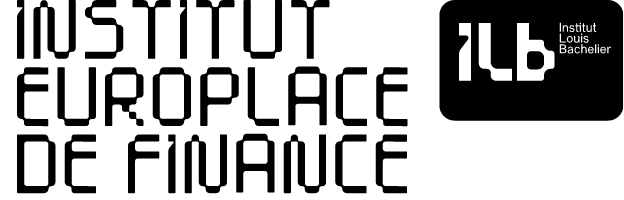
\includegraphics[height=0.9cm]{logos/ilb.png}
        
    \end{center}
\end{frame}

% -----------------------------------------------------------------------------
\begin{frame}{Internship update and topic clarification}
\begin{block}{MVA defense}
  Took place on August 26th 2026, with Alain Oliviero-Durmus and Samy Mekkaoui. Only the CentraleSupélec defense is left, on November 5th 2026.
\end{block}

\begin{block}{Original framing}
Numerical resolution of mean-field games and control with heterogeneous agents using deep learning.
\end{block}
\begin{itemize}
  \item Very broad: MFG + MFC, heterogeneous agents, deep learning.
  \item Too many directions for a focused internship contribution.
\end{itemize}

\begin{block}{Current framing}
Reinforcement learning for mean-field control.
\end{block}
\begin{itemize}
  \item Cooperative, exchangeable population.
  \item Model-free policy gradients.
  \item Perturb the population law through transport / encoding-decoding.
\end{itemize}
\end{frame}

% -----------------------------------------------------------------------------
\begin{frame}{Table of contents}
\tableofcontents
\end{frame}

\section{From classical RL to mean-field control}
% -----------------------------------------------------------------------------
\begin{frame}{Classical RL: the policy-gradient loop}
\begin{center}
  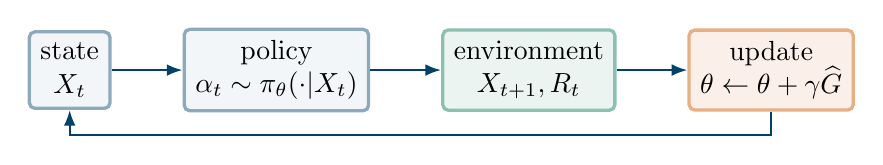
\begin{tikzpicture}[node distance=0.9cm]
  \node[nodebox] (s) {state\\$X_t$};
  \node[nodebox, right=of s] (p) {policy\\$\alpha_t\sim\pi_\theta(\cdot|X_t)$};
  \node[greenbox, right=of p] (e) {environment\\$X_{t+1},R_t$};
  \node[orangebox, right=of e] (u) {update\\$\theta\leftarrow \theta+\gamma \widehat G$};
  \draw[flow] (s) -- (p);
  \draw[flow] (p) -- (e);
  \draw[flow] (e) -- (u);
  \draw[flow] (u.south) |- ++(0,-0.3) -| (s.south);
\end{tikzpicture}
\end{center}

\begin{align*}
  X_0 \sim \mu_0\longrightarrow
  \begin{cases}
    \alpha_t \sim \pi_\theta(\cdot|X_t),\\
    X_{t+1} \sim P_t(\cdot|X_t,\alpha_t),\longrightarrow\\
    R_t = r_t(X_t,\alpha_t),
  \end{cases}
  J(\theta) = \E\left[\sum_{t=0}^{T-1} R_t(X_t, \alpha_t) + g(X_T)\right].
\end{align*}

\begin{block}{REINFORCE identity \cite{williams1992reinforce}}
\[
  \nabla_\theta J(\theta)
  =\E\left[\sum_{t=0}^{T-1}G_t\,\nabla_\theta\log \pi_\theta(\alpha_t|X_t)\right].
\]
\end{block}
\begin{itemize}
  \item $G_t$ is the return-to-go.
  \item No derivative of the transition kernel appears.
  \item This is the basic model-free mechanism.
\end{itemize}
\end{frame}

% -----------------------------------------------------------------------------
\begin{frame}{Mean-field control}

\begin{block}{Large cooperative population}
With exchangeability, pairwise interactions are replaced by the empirical population law. In the limit, one studies a representative agent interacting with $\mu_t$.
\end{block}
\[
  \mu_t^\theta = \Law(X_t^\theta),\qquad
  \alpha_t^\theta\sim\pi_t^\theta(\cdot|X_t^\theta,\mu_t^\theta),
\]
\[
  X_{t+1}^\theta\sim P_t(\cdot|X_t^\theta,\mu_t^\theta,\alpha_t^\theta).
\]
\begin{center}
  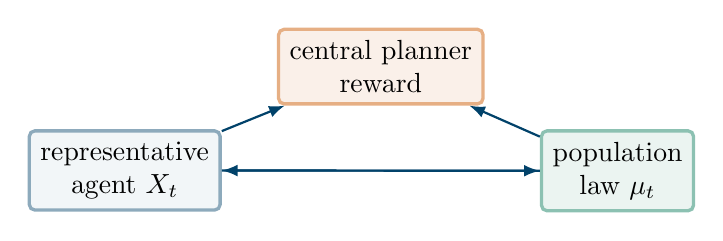
\begin{tikzpicture}[node distance=0.3cm and 0.7cm]
  \node[orangebox] (reward) {central planner\\reward};
  \node[nodebox, below left=of reward] (agent) {representative\\agent $X_t$};
  \node[greenbox, below right=of reward] (law) {population\\law $\mu_t$};

  \draw[flow] (agent) -- (law);
  \draw[flow] (law) -- (agent);
  \draw[flow] (agent) -- (reward);
  \draw[flow] (law) -- (reward);
\end{tikzpicture}
\end{center}

\begin{alertblock}{Distinction from mean-field games}
This is mean-field control: a central planner optimizes a cooperative population objective, not a Nash equilibrium.
\end{alertblock}
\end{frame}

\section{Transport perturbations}
% -----------------------------------------------------------------------------
\begin{frame}{Why classical REINFORCE fails in MFC}
\begin{block}{Objective}
\[
J(\theta)=\E\left[\sum_{t=0}^{T-1}r_t(X_t^\theta,\mu_t^\theta,\alpha_t^\theta)
+g(X_T^\theta,\mu_T^\theta)\right].
\]
\end{block}

\begin{block}{Mean-field dependence}
The exogenous flow $\mu_t^\theta$ depends on $\theta$.
Let $D_t^\theta=\nabla_\theta\mu_t^\theta$, with $D_0^\theta=0$, and define $\bar r_t^\theta(m)\coloneqq\int r_t(x,m,a)\pi_t^\theta(\d a\mid x,m)m(\d x)$ and $\bar g(m)\coloneqq\int g(x,m)m(\d x)$. Then
  \[
  \mu_{t+1}^\theta=\Phi_t^\theta(\mu_t^\theta),
  \qquad
  D_{t+1}^\theta
  =\partial_\theta\Phi_t^\theta(\mu_t^\theta)
  +D_m\Phi_t^\theta(\mu_t^\theta)[D_t^\theta].
\]
and we have the exact gradient formula
\[
  \nabla_\theta J(\theta)
  =\sum_{t=0}^{T-1}
  \left(\partial_\theta\bar r_t^\theta(\mu_t^\theta)
  +D_m\bar r_t^\theta(\mu_t^\theta)[D_t^\theta]\right)
  +D_m\bar g(\mu_T^\theta)[D_T^\theta].
\]
\end{block}

\bad{REINFORCE estimates the direct policy-score term
$\partial_\theta\bar r_t^\theta$, but misses the terms carried by
$D_t^\theta=\nabla_\theta\mu_t^\theta$.}

\end{frame}

% -----------------------------------------------------------------------------
\begin{frame}{Core idea: perturb the law}
\begin{exhibit}{Encode $\longrightarrow$ perturb $\longrightarrow$ decode}
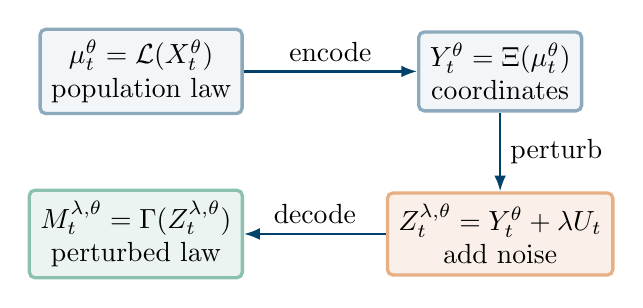
\begin{tikzpicture}
  \node[nodebox] (m) {$\mu_t^\theta = \mathcal L(X_t^\theta)$\\population law};
  \node[nodebox, right=2.2cm of m] (y)
    {$Y_t^\theta= \Xi(\mu_t^\theta)$\\coordinates};
  \node[orangebox, below=1.0cm of y] (z)
    {$Z_t^{\lambda,\theta}=Y_t^\theta+\lambda U_t$\\add noise};
  \node[greenbox, left=1.8cm of z] (mt)
    {$M_t^{\lambda,\theta}=\Gamma(Z_t^{\lambda,\theta})$\\perturbed law};

  \draw[flow] (m) -- node[above]{encode} (y);
  \draw[flow] (y) -- node[right]{perturb} (z);
  \draw[flow] (z) -- node[above]{decode} (mt);
\end{tikzpicture}
\end{exhibit}
\vspace{0.5cm}
\begin{block}{Why this is model-free}
The perturbation density is known. Differentiation with respect to $\theta$ can be transferred to a score of the perturbation variable instead of differentiating the simulator in the measure argument.
\end{block}
\[
  \nabla_\theta\log q_\lambda(Z_t;Y_t^\theta)
  = (D_t^\theta)^\top \nabla_y \log q_\lambda(Z_t;Y_t^\theta),
  \qquad D_t^\theta=\nabla_\theta Y_t^\theta.
\]
\end{frame}

% -----------------------------------------------------------------------------
\begin{frame}{Discrete state: perturb inside the simplex}
Let $\Xc=\{1,\ldots,N\}$ and $\mu_t^\theta\in\Delta_N$, where $\Delta_N = \{p\in\R^N_+: \sum_{i=1}^N p_i=1\}$. We have
\[
  Y_t^\theta=\Xi(\mu_t^\theta)=\mu_t^\theta,\qquad
  \Gamma_\lambda(y,q)=(1-\lambda)y+\lambda q,\qquad
  q_t=\operatorname{softmax}(U_t^{(1)},\ldots,U_t^{(N-1)},0).
\]
Here $U_t\sim\Nc(0,I_{N-1})$, independently across time.

\begin{block}{Boundary-safe perturbation}
Sample $q_t\in\Delta_N^\circ$ from a smooth known law and set
\[
  M_t^{\lambda,\theta}=(1-\lambda)\mu_t^\theta+\lambda q_t,
  \qquad \lambda\in(0,1).
\]
Then, for every $\omega\in\Omega$,
\[
  \TV(M_t^{\lambda,\theta}(\omega),\mu_t^\theta)\leq \lambda.
\]
\end{block}

\begin{block}{Perturbed policy-gradient representation}
\[
  \nabla_\theta J^\lambda(\theta)
  =\E\Big[(\Rc_\theta^\lambda-b_0)
  \big(\Sc_{\mathrm{pol}}^{\lambda,\theta}+\Sc_{\mathrm{mf}}^{\lambda,\theta}\big)\Big].
\]
Here $\Sc_{\mathrm{pol}}$ is the usual policy score and $\Sc_{\mathrm{mf}}$ is a known perturbation-score term multiplied by $D_t^\theta=\nabla_\theta\mu_t^\theta$.
\end{block}
\end{frame}

% -----------------------------------------------------------------------------
\begin{frame}{Continuous state: finite-dimensional population coordinates}
\textbf{Obstacle.}
For $\Xc\subset\R^d$, the law $\mu_t$ lives in an infinite-dimensional space $\Pc(\Xc)$.

\begin{block}{Representation}
Choose coordinates $Y_t^\theta = \Xi(\mu_t^\theta) \in\R^q$ and a decoder $\Gamma$ such that $\mu_t^\theta\approx \Gamma(Y_t^\theta)$.
Examples: Gaussian moments; $K$-Gaussian mixtures.
\end{block}

\begin{block}{Gaussian perturbation}
\[
  Z_t^{\lambda,\theta}=Y_t^\theta+\lambda U_t,
  \qquad U_t\sim\Nc(0,I_q),
\]
\[
  M_t^{\lambda,\theta}=\Gamma(Z_t^{\lambda,\theta}).
\]
The mean-field score is
\[
  \Sc_{\mathrm{mf}}^{\lambda,\theta}
  =\sum_{t=0}^T (D_t^\theta)^\top
  \nabla_y\log q_\lambda(Z_t^{\lambda,\theta};Y_t^\theta)
  =\frac1\lambda\sum_{t=0}^T(D_t^\theta)^\top U_t,
  \qquad D_t^\theta=\nabla_\theta Y_t^\theta.
\]
\end{block}

\begin{alertblock}{Representation of the continuous law}
The strongest result is for stable families, e.g. Gaussian moment closure. Projected/GMM representations add an explicit representation error.
\end{alertblock}
\end{frame}

\section{Guarantees and estimator}
% -----------------------------------------------------------------------------
\begin{frame}{Main result 1: perturbation estimate and consistency}
\begin{block}{Closeness of objectives and gradients}
For suitable regularity constants, uniformly in $\theta$,
\[
  |J^\lambda(\theta)-J(\theta)|\leq C_T\lambda,
  \qquad
  \|\nabla_\theta J^\lambda(\theta)-\nabla_\theta J(\theta)\|\leq C_T^\nabla\lambda.
\]
\end{block}
\begin{block}{Optimizer consistency}
If $\Theta$ is compact, every accumulation point of maximizers of $J^\lambda$ is a maximizer of $J$. If the maximizer is unique,
\[
  \theta_\lambda^\star\longrightarrow \theta^\star.
\]
\end{block}

\good{Solving the perturbed problem is mathematically controlled, not just a heuristic surrogate.}
\end{frame}

% -----------------------------------------------------------------------------
\begin{frame}{Main result 2: estimating the population sensitivity}
The gradient formula still contains $D_t^\theta=\nabla_\theta Y_t^\theta$ or $\nabla_\theta\mu_t^\theta$.
\begin{block}{Recursive auxiliary estimator}
Use a second perturbation radius $\eta$ and $n$ auxiliary trajectories to estimate $D_t^\theta$ recursively.
\[
  \max_{t\leq T}\E\|\widehat D_t^{\eta,M,n,\theta}-D_t^\theta\|_{\mathrm F}^2
  \leq C\left(\eta^2+\frac{1}{n\eta^2}+\frac{1}{M}\right).
\]
\end{block}
\begin{itemize}
  \item $\eta^2$: auxiliary perturbation bias.
  \item $1/(n\eta^2)$: Monte Carlo variance amplified by the score.
  \item $1/M$: population-flow estimation error.
\end{itemize}
\end{frame}

% -----------------------------------------------------------------------------
\begin{frame}{Main result 3: MSE bound for the gradient estimator}
Using $B$ main perturbed trajectories and plugging in $\widehat D_t$ gives
\begin{block}{Bias}
\[
  \big\|\E[\widehat G_{\lambda,\eta,B,M,n}(\theta)]-\nabla_\theta J(\theta)\big\|
  \leq C\left(\lambda+\eta+\frac{1}{\sqrt n\eta}+\frac1{\sqrt M}\right).
\]
\end{block}
\begin{block}{Mean-square error}
\[
  \E\|\widehat G_{\lambda,\eta,B,M,n}(\theta)-\nabla_\theta J(\theta)\|^2
  \leq C\left[\lambda^2+\frac{1+\frac{1}{\lambda^2}}{B}
  +\eta^2+\frac{1}{n\eta^2}+\frac1M\right].
\]
\end{block}
\begin{center}
\small
Choose $\eta\asymp n^{-1/4}$ to balance the auxiliary perturbation terms.
\end{center}
\end{frame}

% -----------------------------------------------------------------------------
\begin{frame}{Algorithm idea: Transport REINFORCE}
\begin{block}{Scores used by the estimator}
\[
  \widehat\Sc_{\mathrm{pol}}^{(b)}
  =\sum_{t=0}^{T-1}\nabla_\theta
  \log p_t^\theta(\widehat\alpha_t^{(b)}|\widehat X_t^{(b)},\widehat M_t^{(b)}),
  \qquad
  \widehat\Sc_{\mathrm{mf}}^{(b)}
  =\sum_{t=0}^T \widehat D_t^\top
  \nabla_y\log q_\lambda(\widehat Z_t^{(b)};\widehat Y_t).
\]
\[
  \widehat G = \frac1B\sum_{b=1}^B
  (\widehat R^{(b)}-b_0)
  \left(\widehat\Sc_{\mathrm{pol}}^{(b)}+
  \widehat\Sc_{\mathrm{mf}}^{(b)}\right).
\]
\end{block}

\textbf{One policy update.}
\begin{enumerate}
  \item Simulate a population batch and estimate $\widehat Y_{0:T}$.
  \item Set $\widehat D_0=0$ and estimate $\widehat D_1,\ldots,\widehat D_T$ recursively with auxiliary perturbations at $\eta$.
  \item Simulate $B$ main perturbed trajectories at $\lambda$.
  \item Form $\widehat G$ from the policy and mean-field scores, then update $\theta\leftarrow\theta+\gamma\widehat G$.
\end{enumerate}

\begin{alertblock}{Implementation note}
Experiments use a shared-batch implementation with simulator cost
\[
  C_{\mathrm{sim}}^{\mathrm{shared}}=T(M+n+B).
\]
\end{alertblock}
\end{frame}

\section{Benchmarks}
% -----------------------------------------------------------------------------
\begin{frame}{Benchmark: mean--variance portfolio}
This is the cleanest continuous benchmark for explaining the additional mean-field term.

\begin{block}{Dynamics and rewards}
\[
  X_{t+1}=s_tX_t+\alpha_t R_{t+1}.
\]
\[
  r(x,a,\mu)=-\gamma\,m(\mu)^2,
  \qquad
  g(x,\mu)=x-\chi(x-m(\mu))^2,
\]
\[
  m(\mu)=\int x\,\mu(\d x)
  \quad\text{is the population mean wealth.}
\]
\end{block}
\begin{block}{Policy class}
\[
  \alpha_t=k_t(X_t-m_t)+\ell_t+\tau_t\varepsilon_t.
\]
Moment recursions are exact, so validation has no trajectory noise.
\end{block}

\begin{alertblock}{Implementation notes}
  \begin{itemize}
    \item The algorithm used is an older version, a new algorithm based on the updated continuous-state theory is being implemented.
    \item The following results are only illustrative of the mean-field score effect, some ML/optimization effects are being tuned.
  \end{itemize}
\end{alertblock}

\end{frame}

% -----------------------------------------------------------------------------
\begin{frame}{Portfolio: training}
\small
\begin{exhibit}{Validation reward over training}
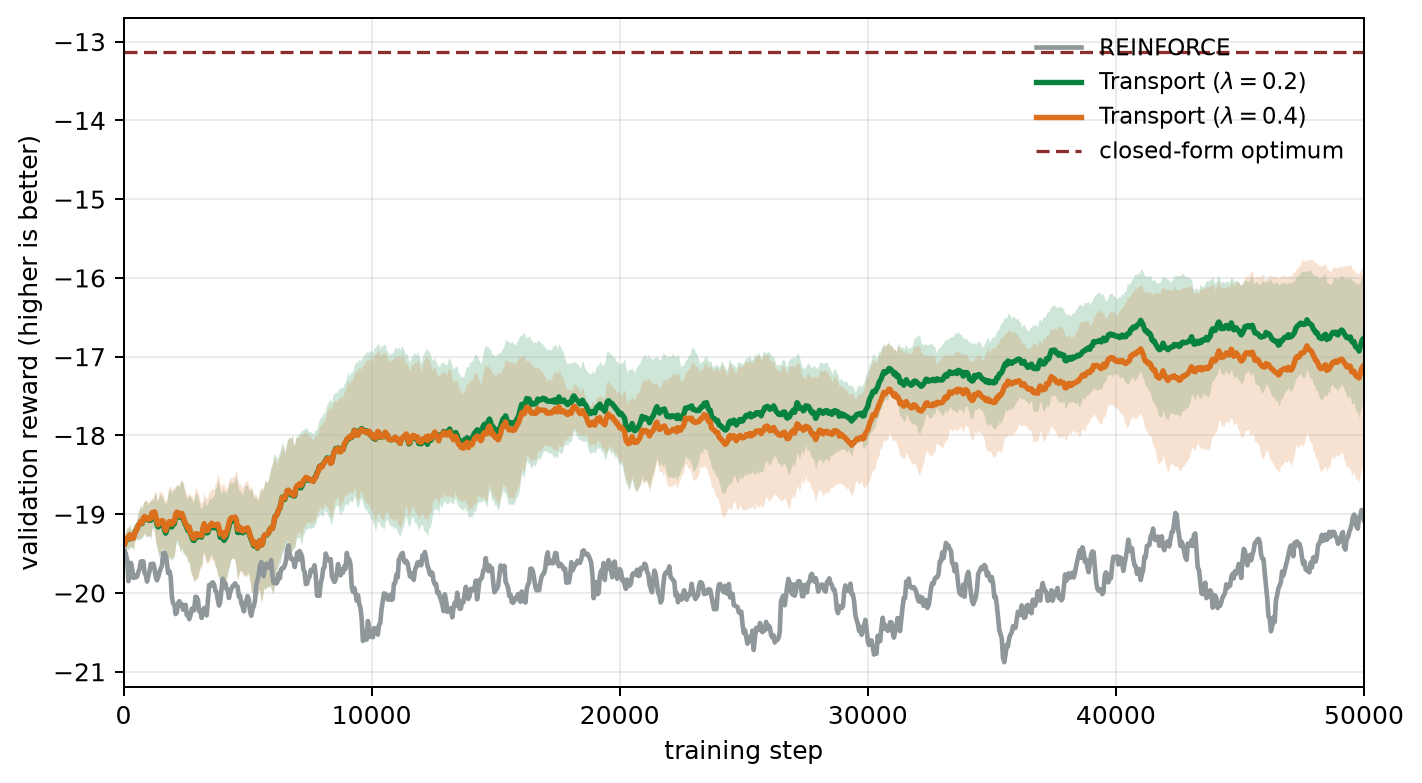
\includegraphics[width=0.78\linewidth]{portfolio_validation_fixed_T10_50k.png}
\end{exhibit}
\exhibitnote{Mean and one standard deviation over five seeds at $T=10$. Higher objective is better.}

\vspace{0.1cm}
Fixed transport continues improving at 50k steps, with $\lambda=0.2$ giving the cleanest final result. Standard REINFORCE does not recover the missing mean-field direction.
\end{frame}

% -----------------------------------------------------------------------------
\begin{frame}{Portfolio: final validation result}
\small
\begin{exhibit}{Final validation result}
\begin{tabular}{lrrr}
\toprule
Method & Objective & Gap & $\|\nabla J\|$ \\
\midrule
Optimum & $-13.133$ & $0$ & $0.000$ \\
REINFORCE & $-19.077$ & $5.944$ & $1.273$ \\
Transport, $\lambda=0.2$ & $\mathbf{-16.762}$ & $\mathbf{3.629}$ & $\mathbf{0.796}$ \\
Transport, $\lambda=0.4$ & $-17.109$ & $3.976$ & $0.838$ \\
\bottomrule
\end{tabular}
\end{exhibit}
\exhibitnote{Mean over five seeds at $T=10$. Higher objective is better; the gap is $|J(\widehat\theta)-J(\theta^\star)|$. The gradient norm is exact, from the closed-form moment recursion.}

\vspace{0.2cm}
The exact optimum of the perturbed $\lambda=0.2$ problem is $-13.173$. The bottleneck is the optimization of the perturbed problem, not the perturbation itself. The mean-field score helps the optimizer find a better local optimum. Likely causes include
\begin{itemize}
  \item Finite noisy gradient estimates.
  \item Constant Adam \cite{kingma2014adam} learning rate.
  \item Fixed finite $\eta=0.85$, not controlled with sample size as the theory suggests.
  \item No asymptotic decay of $\lambda$ to zero.
\end{itemize}
\end{frame}

% -----------------------------------------------------------------------------


% -----------------------------------------------------------------------------
\begin{frame}{The mean-field term ablation}
The reward is written as:
\begin{align*}
  r(x,\mu,a) = -\gamma m(\mu)^2, \qquad g(x,\mu) = x - \chi(x-m(\mu))^2.
\end{align*}

\vspace{0.05cm}
The coefficient $\gamma$ multiplies the only direct running reward term that depends on the population mean. Switching it off keeps the dynamics, policy class, seeds and simulator budgets fixed.

\vspace{0.15cm}
\scriptsize
\begin{exhibit}{Controlled pair: population channel off and on}
\begin{tabular}{lrrl}
\toprule
Setting & $\|G_{\rm full}\|$ & $\varrho(G_{\rm full},G_{\rm det})$ & Outcome \\
\midrule
$\gamma=0$ & $0.083$ & $+1.000$ & correction unnecessary \\
$\gamma=2$ & $1.357$ & $-0.196$ & correction changes direction \\
\bottomrule
\end{tabular}
\end{exhibit}
\exhibitnote{$G_{\rm det}$ is the gradient estimated by standard REINFORCE; $\varrho$ is its cosine alignment with the full mean-field gradient.}

\vspace{0.15cm}
\small
At $\gamma=0$, REINFORCE is directionally correct. At $\gamma=2$, the detached gradient is nearly orthogonal and slightly opposed to the full gradient, which explains why the mean-field score becomes useful.
\end{frame}

% -----------------------------------------------------------------------------
\begin{frame}{Other benchmarks and comparisons}
\begin{table}
\centering
\small
\begin{tabular}{lll}
\toprule
Benchmark & Type & Role in the paper \\
\midrule
Two-state control \cite{meunier2026model,gu2023dynamic} & finite & sanity check; explicit optimal policy \\
Cybersecurity \cite{meunier2026model,kolokoltsov2016mean,carmona2023model} & finite & comparison with other methods \\
Distribution planning \cite{meunier2026model,carmona2023model} & finite & higher-dimensional simplex transport \\
Targeted advertising \cite{motte2021mathematical} & finite & population control example \\
Linear--quadratic control & continuous & Gaussian closure and exact oracle \\
Portfolio \cite{cui_li_li_mean_variance,fischer_livieri_mean_variance} & continuous & gamma ablation; clean MF reward term \\
\bottomrule
\end{tabular}
\end{table}

For all benchmarks, we compare with REINFORCE. In discrete-state benchmarks, we also compare with MF-REINFORCE \cite{meunier2026model} (all four benchmarks) and MF $Q$-learning \cite{carmona2023model} (cybersecurity).

\end{frame}

\section{Positioning and next steps}
% -----------------------------------------------------------------------------
\begin{frame}{Related works}
\begin{block}{Meunier--Pham--Reisinger policy-gradient perturbation \cite{meunier2026model}}
Their finite-state method perturbs log-probabilities and uses a softmax decoder:
\[
  \mu^\varepsilon=\operatorname{softmax}(\log\mu+\varepsilon\Lambda).
\]
In our framework, this is a coordinate perturbation with $\Xi=\log$ and $\Gamma=\operatorname{softmax}$.
\end{block}

\begin{itemize}
  \item It is tied to finite probability vectors; continuous laws need a finite-dimensional representation before they can be perturbed.
  \item The log map is singular at the simplex boundary, whereas the convex perturbation above stays well defined even when some masses vanish.
\end{itemize}

\begin{block}{Value-based alternative \cite{carmona2023model}}
MFMDP $Q$-learning lifts the state to the population law. It is conceptually natural, but simplex discretization scales poorly.
\end{block}
\end{frame}

% -----------------------------------------------------------------------------
  
% -----------------------------------------------------------------------------
\begin{frame}{Future work before final delivery}
\begin{block}{Current goal}
  Submit to ICLR 2027 before the 24th of September.
\end{block}

\begin{enumerate}
  \item Proof-read the statements and their proofs.
  \item Freeze the numerical experiment suite and identify the final plots/results.
  \item Run and analyze the final experiments.
  \item Finalize the paper and submit.
\end{enumerate}

\begin{block}{Final presentation}
  Thursday, November 5th, 14:45 -- 15:45.
\end{block}
\end{frame}

% -----------------------------------------------------------------------------
\begin{frame}[allowframebreaks]{References}
\printbibliography
\end{frame}

\end{document}
